\documentclass[a4paper]{article}
%\documentclass[12pt]{iopart}
%% Language and font encodings
\usepackage[english]{babel}
\usepackage[utf8x]{inputenc}
\usepackage[T1]{fontenc}
\usepackage[title]{appendix}
\usepackage{authblk}
\usepackage{siunitx}

%% Sets page size and margins
\usepackage[a4paper,top=3cm,bottom=3cm,left=3cm,right=3cm,marginparwidth=1.75cm]{geometry}

%% Useful packages
\usepackage{amsmath}
\usepackage{graphicx}
\usepackage[colorinlistoftodos]{todonotes}
\usepackage[colorlinks=true, allcolors=blue]{hyperref}
\usepackage{subfig}
\usepackage[parfill]{parskip}
\usepackage{float}
\usepackage{mathtools}

%\begin{document}

%\title{Nutrient-drug coupling can prevent or enhance spatial expansion of a bacterial population}

\renewcommand{\thefigure}{S\arabic{figure}}

\title{Supplementary Material: Growth-dependent drug susceptibility can prevent or enhance spatial expansion of a bacterial population}

%\author{Patrick Sinclair, Mart\'{i}n Carballo Pacheco and Rosalind J Allen}
\author{Patrick Sinclair}
\author{Mart\'{i}n Carballo-Pacheco}
\author{Rosalind J Allen}
\affil{School of Physics and Astronomy, University of Edinburgh,  Peter Guthrie Tait Road, Edinburgh, EH9 3FD, United Kingdom}
\date{}
%\address{}
%\ead{rosalind.allen@ed.ac.uk}

%\keywords{magnetic moment, solar neutrinos, astrophysics}
%\submitto{\PB}

\begin{document}

\maketitle

\section*{Equivalent results are obtained for a steeper antibiotic gradient}

\begin{figure}
\centering
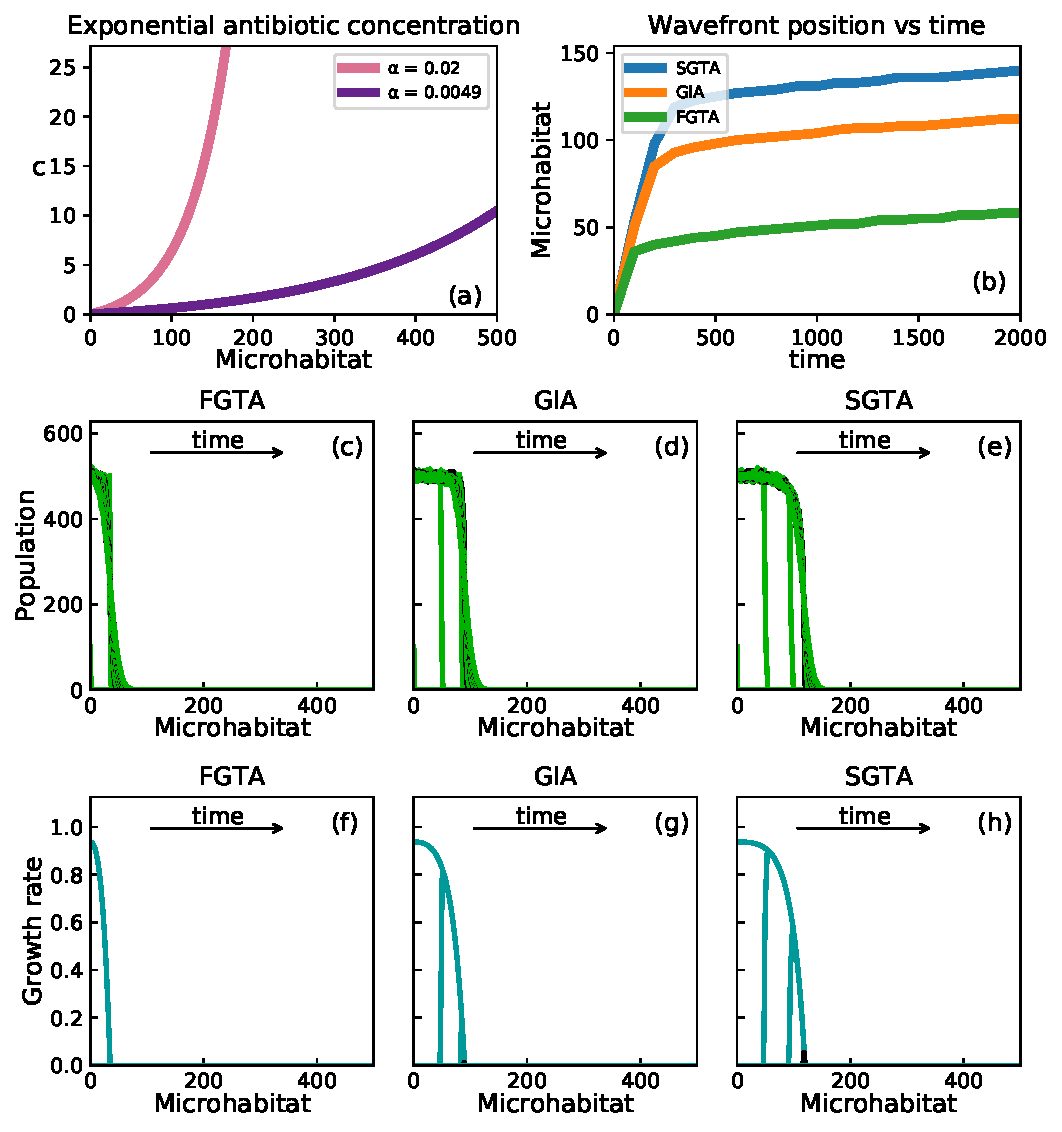
\includegraphics[width=0.9\textwidth]{supplementary_figures_alpha_0_002-FINAL.pdf}[H]
\caption{Population dynamics in a gradient of a bacteriostatic antibiotic for $\alpha=0.02$. (a) Profile of the antibiotic concentration, for $\alpha=0.02$ (pink line, discussed here). The profile for $\alpha=0.00049$ (purple line), discussed in the main text, is also shown here (b) Position of the advancing population wavefront for the three antibiotic types. The waves advance at a constant speed before stopping when the antibiotic concentration prevents bacterial growth.  The SGTA is the least effective at curtailing the spatial advance of the population, followed by GIA and FGTA. (c)-(e) Snapshots of the bacterial population density, sampled every 100 time units (for clarity, every 4th snapshot is shown in black), for the three antibiotic types. The wave spreads further in the SGTA case and less far in the FGTA case. (f)-(h)  Spatial profiles of the local bacterial growth rate ($b_i$), sampled every 100 time units for the three antibiotic types. Black lines here correspond to the same time points as those in panels c-e.}\label{fig:supplementary-material}
\end{figure}

In the main text, we discuss how a bacterial population invades a spatial domain in which the concentration of antibiotic increases exponentially. The results presented in the main text are for a rather shallow antibiotic gradient, with $\alpha=0.0049$ (see figure 3). Here, we repeat our simulations for a steeper antibiotic profile, with 
$\alpha=0.02$ (figure \ref{fig:supplementary-material}). Our conclusions are the same as those presented in the main text. Specifically, we observe a difference in the final position of the population wave depending on the growth-dependent susceptibility of the antibiotic: the wave advances the furthest for SGTA, followed by GIA and FGTA. Compared to our results for 
$\alpha=0.0049$ (main text, figure 3), for $\alpha=0.02$ the population wave advances less far, since it encounters higher antibiotic concentrations earlier. 


\section*{Interplay between growth-dependent susceptibility and the shape of the pharmacodynamic function}

\begin{figure}
\centering
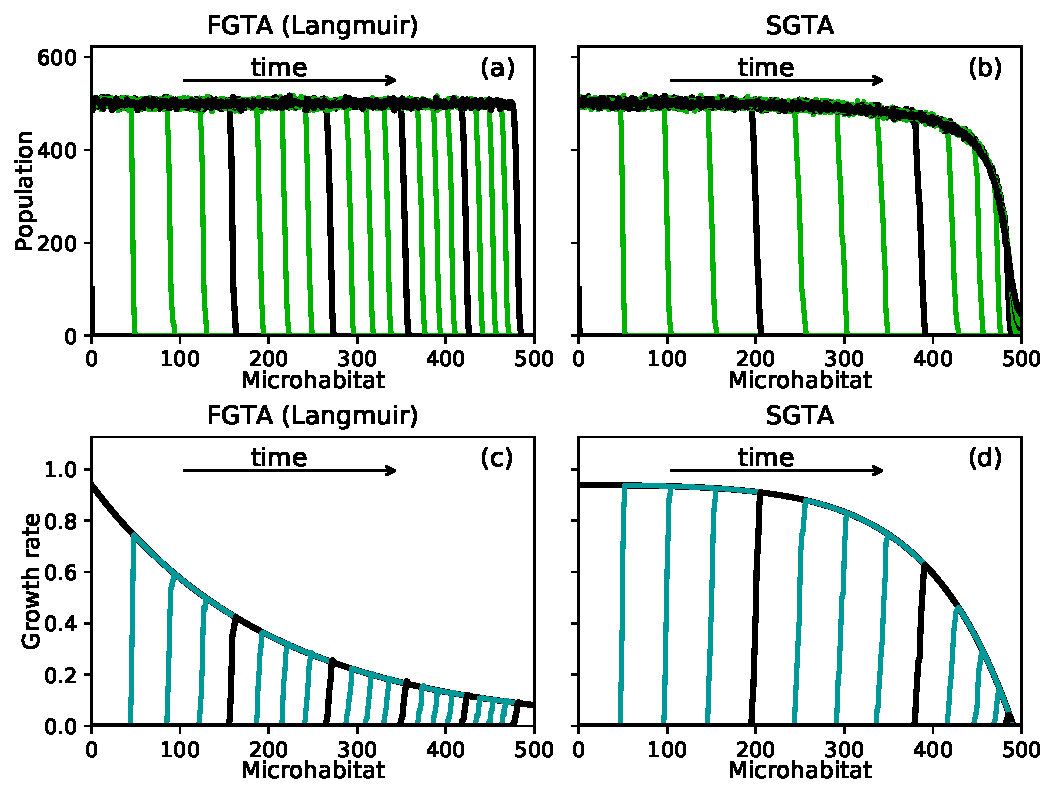
\includegraphics[width=0.9\textwidth]{supplementary_realistic_simple_comparison}[H]
\caption{(a)-(b) Population density and (c)-(d) growth rate profiles, for (left): an FGTA growth-dependent susceptibility combined with a Langmuir-like pharmacodynamic function (mimicking tetracycline) and (right): an SGTA growth-dependent susceptibility combined with a quadratic pharmacodynamic function. In all cases, $\alpha=0.0049$.} \label{fig:supplementary-material-real-simple-compare}
\end{figure}

In the main text, we showed that using a Langmuir-like instead of quadratic pharmacodynamic function does not change our conclusion that, for bacteriostatic antibiotics, an FGTA antibiotic is more effective at halting bacterial invasion than an SGTA antibiotic. In making that comparison, we assumed that the shape of the pharmacodynamic function is independent of the growth-dependent susceptibility: i.e. that the same pharmacodynamic function applies to both the FGTA and SGTA antibiotics. However, this may not be true.  In particular, Greulich et al. \cite{Greulich2015} showed that while streptomycin and kanamycin have threshold-like pharmacodynamic functions and are SGTA antibiotics, tetracycline and chloraphenicol have Langmuir-like pharmacodynamic functions and are FGTA antibiotics. Moreover, the mathematical model presented by Greulich et al. suggested that there may be an intrinsic link between growth-dependent suscpetibility and the shape of the pharmacodynamic function \cite{Greulich2015}. In figure \ref{fig:supplementary-material-real-simple-compare}, we "mimic" an experiment in which  an FGTA antibiotic with a Langmuir-like pharmacodynamic function (similar to tetracycline) is compared to an SGTA antibiotic with a quadratic pharmacodynamic function (similar to streptomycin). In these simulations, we see that there is a tradeoff between the effect of the pharmacodynamic function and the growth-dependent susceptibility, with the result that both antibiotics are approximately equally effective at halting the bacterial population wave. From a practical point of view, coupling between the shape of the pharmacodynamic function and growth-dependent susceptibility could complicate experimental tests of the concepts presented in this work.  

\bibliographystyle{unsrt.bst}
\bibliography{literature}

\end{document}